% --------------------------------------------------------------------------------

\begin{exercise}[Exercise 3.24]

Figure \ref{fig:2.21} (below) gives the optimal value of the best state of the gridworld as $24.4$, to one decimal place.
Use your knowledge of the optimal policy and \eqref{eq:2.15} to express this value symbolically, and then to compute it to three decimal places.

\begin{figure}[H]
    \centering
    \subfloat[Gridworld]
    {
        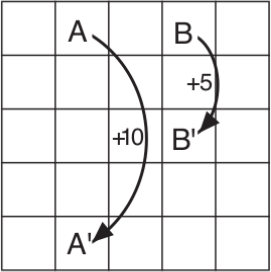
\includegraphics[width = 0.2 \textwidth]{2.21.1.png}
    }
    \hspace{1cm}
    \subfloat[$v_\ast$]
    {
        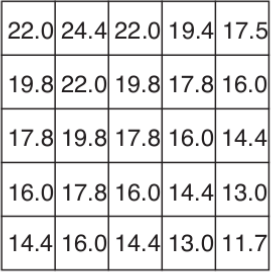
\includegraphics[width = 0.2 \textwidth]{2.21.2.png}
    }
    \hspace{1cm}
    \subfloat[$\pi_\ast$]
    {
        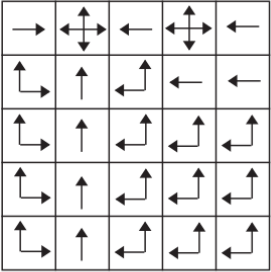
\includegraphics[width = 0.2 \textwidth]{2.21.3.png}
    }
    \hspace{0mm}
    \caption
    {
        Optimal solutions to the gridworld example.
    }
    \label{fig:2.21}
\end{figure}

\end{exercise}

% --------------------------------------------------------------------------------

\begin{solution}

ToDo!

\end{solution}

% --------------------------------------------------------------------------------
